%%  -*- ispell-local-dictionary: "american-w_accents" -*-
\PassOptionsToPackage{dvipsnames}{xcolor}
\documentclass[utf8x]{beamer}
\usepackage[dvipsnames]{xcolor}
\usepackage{etex}
\usepackage[english]{babel}
\usepackage[utf8x]{inputenc}
\usepackage[T1]{fontenc}
\usepackage{amsmath,amsthm,amsfonts}
\usepackage[all, color, pdf]{xy}
\usepackage{mathtools}
%\usepackage{realboxes} % for \Colorbox
\usepackage{skull} % for \skull
%\usepackage{ulem}
\usepackage{marvosym} % for \Lightning
\usepackage{amssymb}
\usepackage{cancel}
\usepackage{fourier} % for \danger
\usepackage[scaled=0.85]{beramono}
\renewcommand{\ttdefault}{pcr}
\usepackage{listings}
\usepackage{lstcoq}
\lstset{language=Coq}
\usepackage{boxedlistings}
\lstset{style=script}

%\lstset{backgroundcolor=\color{black!15}}
%\lstset{basicstyle=\scriptsize\bf\ttfamily,escapeinside={(*@}{@*)}}

\lstset{escapeinside={(*@}{@*)}}

%\usecolortheme{crane}


\setbeamertemplate{navigation symbols}{}
\setbeamercovered{invisible}

\newcommand\hfilll{\hskip 0pt plus 1filll}
\newcommand\cit[1]{\hfill {\scriptsize \textcolor{purple}{[#1]}}}
\newcommand\gris[1]{\uncover{{\color{gray} #1}}}
\newcommand\auteur[2]{#1~\textsc{#2}}
\newcommand\mycite[1]{\textcolor{purple}{#1}}
\newcommand\Checkmark{\textcolor{mygreen}{\checkmark}}
\newcommand<>{\alertb}[1]{\alt#2{\textcolor{blue}{#1}}{#1}}

% Rising dots
\makeatletter
\def\revddots{\mathinner{\mkern1mu\raise\p@
\vbox{\kern7\p@\hbox{.}}\mkern2mu
\raise4\p@\hbox{.}\mkern2mu\raise7\p@\hbox{.}\mkern1mu}}
\makeatother


\title{Formal Proof of a Gathering Algorithm in the Pactole Framework}
\author{\auteur{Mathis}{Bouverot-Dupuis}}
\institute{Boss : Pierre Courtieu (CNAM)}
\date[12 juillet 2022]{June - July 2022}


\begin{document}
\frame{\maketitle}

\begin{frame}
\frametitle{Talk outline}
  \tableofcontents
\end{frame}


\section{Suzuki \& Yamashita's Model}
%%%%%%%%%%%%%%%

\begin{frame}
\frametitle{Suzuki \& Yamashita's Model}
\begin{overlayarea}{\linewidth}{10em}
  
  \begin{minipage}{.6 \linewidth}
    Very simple (dumb) robots :
    \begin{itemize}
      \item<1-> Points in $\mathbb{R}^2$ (can overlap)
      \item<2-> Anonymous
      \item<3-> No direct communication
      \item<4-> No common direction/scale 
      \item<5-> Strong multiplicity detection
      \item<6-> Same robogram
    \end{itemize}
  \end{minipage}
  \hfill
  \begin{minipage}{.38 \linewidth}
    \includegraphics<1-3>[width=\linewidth, keepaspectratio]{figures/points_scattered}
    \includegraphics<4->[width=\linewidth, keepaspectratio]{figures/points_referential}
  \end{minipage}

\end{overlayarea}
\end{frame}

\section{Weber Point Properties}
%%%%%%%%%%%%%%%%%%%%%

\begin{frame}
\frametitle{Weber point : Definition}
\begin{overlayarea}{\linewidth}{20em}

  \begin{itemize}
    \item<1-> Let $X$ : multiset of points in $\mathbb{R}^2$
    \item<2-> Sum of distances to X : 
      $$D_X(p) := \sum_{x \in X} \lVert x - p \rVert$$
    \item<3-> Set of weber points of X : 
      $$\{p \mid p \textrm{ minimizes } D_X\}$$
    \item<4-> Similar to barycenter (sum of distances v.s. sum of distances squared).
  \end{itemize}

\end{overlayarea}
\end{frame}

\begin{frame}
\frametitle{Weber point v.s Barycenter}
\begin{overlayarea}{\linewidth}{20em}

  \vspace{1em}

  \begin{center}
  \begin{tabular}{ |c|c|c| } 
    \hline
           & barycenter & weber point \\ 
    \hline
    exists & \only<2->{Yes} & \only<2->{Yes} \\ 
    \hline
    unique & \only<3->{Yes} & \only<3->{\textcolor{red}{No}} \\ 
    \hline
    computable & \only<4->{Yes} & \only<4->{\textcolor{red}{No}} \\
    \hline
  \end{tabular}
  \end{center}

  \vspace{1em}

  \only<5->{When is the weber point unique ?}
  \begin{itemize}
    \item<6-> Points not aligned.
    \item<7-> Odd number of points.
    \item<8-> Otherwise : sometimes.
  \end{itemize}

  \only<9->{How about computability ?}
  \begin{itemize}
    \item<10-> We don't care (toy example).
  \end{itemize}

  \only<11->{Why use the weber point ?}

\end{overlayarea}
\end{frame}

\begin{frame}
\frametitle{Contraction Lemma}
\begin{overlayarea}{\linewidth}{20em}

  \begin{itemize}
    \item<1-> Let \textcolor{BrickRed}{\bf{X}}, \textcolor{LimeGreen}{\bf{Y}} : multiset of points (cf. figure).
    \item<2-> Suppose \textcolor{blue}{$w$} $\in WP(X)$.
    \item<3-> Then \textcolor{blue}{$w$} $\in WP(Y)$.
  \end{itemize}

  \begin{center}
    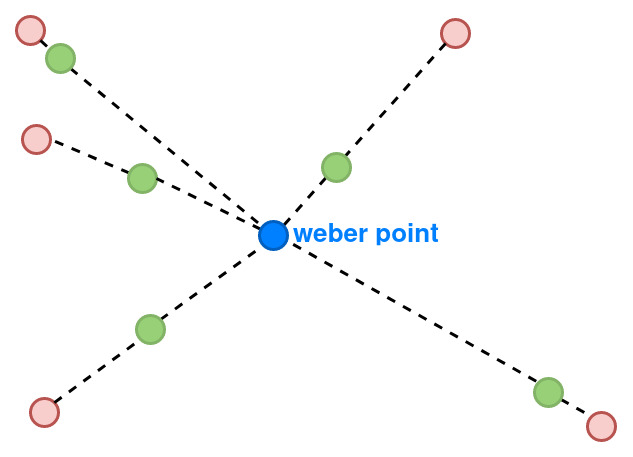
\includegraphics[width=0.7\linewidth, keepaspectratio]{figures/weber_contract}
  \end{center}

\end{overlayarea}
\end{frame}

\begin{frame}
\frametitle{Contraction Lemma (proof idea)}
\begin{overlayarea}{\linewidth}{20em}

  Alternate characterization of weber points :
  \begin{itemize}
    \item<2-> Recall $D_X(p) := \sum_{x \in X} \lVert x - p \rVert$.
    \item<3-> $D_X$ is convex \& differentiable (almost) everywhere.
    \item<4-> Minimizing $D_X$ $\iff$ gradient of $D_x$ is $0$. 
    \item<5-> Gradient : 
      $\nabla D_X(p) = \sum_{x \in X} \frac{p - x}{\lVert p - x \rVert}$
  \end{itemize}
  
  \begin{center}
    \includegraphics<1-4>[width=0.65\linewidth, keepaspectratio]{figures/weber_charact}
    \includegraphics<5->[width=0.65\linewidth, keepaspectratio]{figures/weber_charact_arrows}
  \end{center}

\end{overlayarea}
\end{frame}

\section{Alignment}
%%%%%%%%%%%%%%%

\begin{frame}[fragile]
\frametitle{Alignment}
\begin{overlayarea}{\linewidth}{20em}
   
  Goal : move robots to a common line, and make them stay on the line.
    
  \begin{onlyenv}<1>
    \vspace{2em}
    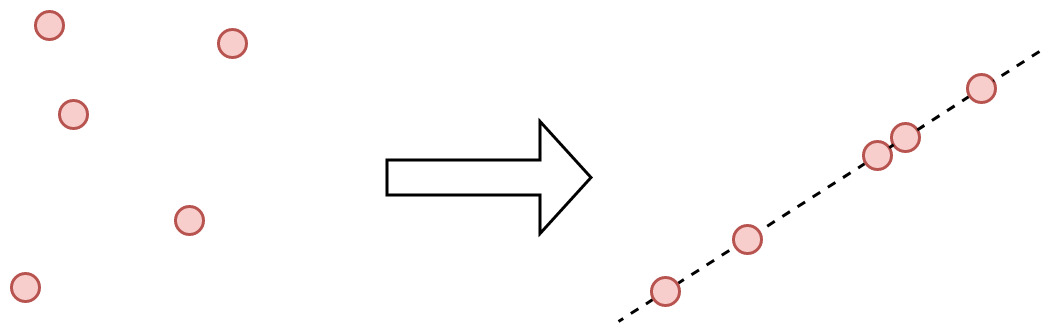
\includegraphics[width=\linewidth, keepaspectratio]{figures/points_align}
  \end{onlyenv}
  
  \begin{onlyenv}<2->
    \begin{lstlistingCoq}
Definition aligned : configuration -> Prop.
    \end{lstlistingCoq}
  \end{onlyenv}

  \begin{onlyenv}<3->
    \begin{lstlistingCoq}
Definition eventually_aligned (c:configuration) 
(d:demon) (r:robogram) := 
  Stream.eventually 
    (Stream.forever (Stream.instant aligned)) 
    (execute r d c).
    \end{lstlistingCoq}
  \end{onlyenv}

  \begin{onlyenv}<4->
    \begin{lstlistingCoq}
Theorem alignment_correct := 
  forall (c:configuration) (d:demon), 
    (* Hypotheses on d *) -> 
    eventually_aligned c d align_robogram.
    \end{lstlistingCoq}
  \end{onlyenv}

\end{overlayarea}
\end{frame}

\begin{frame}[fragile]
\frametitle{Robogram}
\begin{overlayarea}{\linewidth}{10em}

  Very simple robogram : move towards the weber point (in a straight line) until aligned.

  \begin{onlyenv}<2->
    \begin{lstlistingCoq}
Definition align_robogram (obs:observation) : R2 := 
  if aligned_dec obs
  then origin 
  else weber_calc obs.
  \end{lstlistingCoq}
  \end{onlyenv}

  \begin{onlyenv}<3->
    \begin{lstlistingCoq}
Definition observation := multiset R2.
    \end{lstlistingCoq}
  \end{onlyenv}

\end{overlayarea}
\end{frame}

\begin{frame}
\frametitle{Setting}
\begin{overlayarea}{\linewidth}{10em}

  Suzuki \& Yamashita's Model : several versions.
  \begin{itemize}
    \item<1-> Fully-synchronous (FSYNC), semi-synchronous (SSYNC) or asynchronous (ASYNC) ?
    \item<2-> Rigid or flexible ?
  \end{itemize}

  \only<3->{My proofs (alignment) :} 
  \begin{itemize}
    \item<4-> SSYNC \& rigid.
    \item<5-> SSYNC \& flexible.
    \item<6-> ASYNC (first time in Pactole) \& flexible.
  \end{itemize}

\end{overlayarea}
\end{frame}

\begin{frame}[fragile]
\frametitle{ASYNC model}
\begin{overlayarea}{\linewidth}{20em}

  How do we represent robots ?
  \begin{itemize}
    \item<2-> SSYNC : current position only.
    \item<3-> ASYNC : start, destination \& current positions.
  \end{itemize}

  \begin{onlyenv}<4->
    \begin{lstlistingCoq}
Definition info := (location * location * ratio)%type.
    \end{lstlistingCoq}
  \end{onlyenv}

  \begin{onlyenv}<5->
    \begin{lstlistingCoq}
Instance St : State info := 
{ get_location := fun '(start, dest, r) => 
    straight_path start dest r }.
    \end{lstlistingCoq}
  \end{onlyenv}

  \only<6->{How to update robots each round ?} 
  \begin{itemize}
    \item<7-> Activated robots : 
      \begin{lstlisting}
new_start <- straight_path start dest ratio
new_dest  <- robogram (obs_from_config config)
new_ratio <- 0
      \end{lstlisting}
    \item<8-> Other robots : 
      \begin{lstlisting}
new_ratio <- ratio + demon_ratio
      \end{lstlisting}
  \end{itemize}

  \only<8->{\textbf{obs\_from\_config} forgets the start and destination.}
  
\end{overlayarea}
\end{frame}

\begin{frame}[fragile]
\frametitle{ASYNC model : rigid \& flexible}
\begin{overlayarea}{\linewidth}{15em}
  
  How to define rigid \& flexible demons in ASYNC ?  
  \vspace{1em}

  \begin{onlyenv}<2->
    Rigid : no longer the default setting.
    \begin{lstlistingCoq}
Definition rigid_da_prop (da:demonic_action) :=
  forall (c:configuration) (id:ident),
    da.(activate) id = true -> 
    get_location (c id) == get_destination (c id).
    \end{lstlistingCoq}
  \end{onlyenv}

  \begin{onlyenv}<3->
    Flexible :
    \begin{lstlistingCoq}
Definition flex_da_prop (da:demonic_action) (delta:R) :=
  forall (c:configuration) (id:ident),
    da.(activate) id = true -> 
    get_location (c id) == get_destination (c id) \/
    delta <= dist (get_start (c id)) (get_location (c id)).
    \end{lstlistingCoq}
  \end{onlyenv}

\end{overlayarea}
\end{frame}


\begin{frame}[fragile]
\frametitle{Decreasing measure}
\begin{overlayarea}{\linewidth}{15em}
  
  We define a measure that decreases each time a robot that isn't on the weber point is activated.
  
  \begin{itemize}
    \item<1-> Simple case : SSYNC \& rigid.
    \item<2-> Count how many robots have not arrived yet.
  \end{itemize}

  \begin{onlyenv}<3-> 
    \begin{lstlistingCoq}
Definition measure (c:configuration) :=
  n - countA_occ _ _ (weber_calc c) c.
    \end{lstlistingCoq}
  \end{onlyenv} 
  
  \begin{onlyenv}<4-> 
    \begin{lstlistingCoq}
Lemma round_decreases_measure :
  forall (c:config) (da:demonic_action), 
    (* Hypotheses on da *) ->
    (exists id, da.(activate) id = true /\ 
      get_location (c id) =/= weber_calc c) -> 
    aligned (round gatherW da c).
    \end{lstlistingCoq}
  \end{onlyenv}

\end{overlayarea}
\end{frame}

\begin{frame}
\frametitle{Decreasing measure (ASYNC \& flex)}
\begin{overlayarea}{\linewidth}{20em}
  
  Lifecycle of a robot in ASYNC flex : \\
  \begin{minipage}{0.32 \linewidth}
    \includegraphics<2->[width=0.9\linewidth, keepaspectratio]{figures/activate_first}
  \end{minipage}
  \begin{minipage}{0.32 \linewidth}
    \includegraphics<3->[width=0.9\linewidth, keepaspectratio]{figures/activate_second}
  \end{minipage}
  \begin{minipage}{0.32 \linewidth}
    \includegraphics<4->[width=0.9\linewidth, keepaspectratio]{figures/activate_third}
  \end{minipage}

\end{overlayarea}
\end{frame}

\begin{frame}[fragile]
\frametitle{Decreasing measure (ASYNC \& flex)}
\begin{overlayarea}{\linewidth}{20em}
    
  We need one measure for each type of activation. 

  \begin{itemize}
    \item<2-> \textbf{measure\textsubscript{1}} : count how many robots are looping but not on the weber point. 
    \item<3-> \textbf{measure\textsubscript{2}} : count the total distance from the start of each robot to the weber point. 
    \item<4-> \textbf{measure\textsubscript{3}} : count how many robots are \textbf{not} looping on the weber point.  
  \end{itemize}

  \only<5->{The final measure is $\textbf{measure\textsubscript{1}} + \textbf{measure\textsubscript{2}} + \textbf{measure\textsubscript{3}}$.}
  
  \only<6->{The proof is then a well-founded induction on the measure.}

  \begin{onlyenv}<7-> 
    \begin{lstlistingCoq}
Definition lt_config (c1 c2:configuration) :=
  0 <= measure c1 <= measure c2 - min 1 delta.
    \end{lstlistingCoq}
  \end{onlyenv}

  \begin{onlyenv}<8-> 
    \begin{lstlistingCoq}
Lemma lt_config_wf : well_founded lt_config.
    \end{lstlistingCoq}
  \end{onlyenv}

\end{overlayarea}
\end{frame}


\section{Gathering}
%%%%%%%%%%%%%%%%%%%


\begin{frame}[fragile]
\frametitle{Gathering}
\begin{overlayarea}{\linewidth}{20em}

  \vspace{1em}

  Does the algorithm work for gathering ? 
  \pause
  \begin{itemize}
    \item Problem when aligned : weber point is not unique.
  \end{itemize}
  \pause 
  Switch to another algorithm once aligned ?
  \pause 
  \begin{itemize}
    \item Does not work in ASYNC. 
  \end{itemize}
  \pause
  For which initial configurations does the weber algorithm work ?
  \pause
  \begin{itemize}
    \item When the weber point is unique (initially).
  \end{itemize}

\end{overlayarea}
\end{frame}
  
\begin{frame}
\frametitle{Strong Contraction Lemma (Zohir Bouzid)}
\begin{overlayarea}{\linewidth}{20em}
  
  \begin{itemize}
    \item<1-> Let \textcolor{BrickRed}{\bf{X}}, \textcolor{LimeGreen}{\bf{Y}} : multiset of points (cf. figure).
    \item<2-> Suppose \textcolor{blue}{$w$} is the \textbf{\textcolor{red}{unique}} weber point of $X$.
    \item<3-> Then \textcolor{blue}{$w$} is the \textbf{\textcolor{red}{unique}} weber point of $Y$.
  \end{itemize}

  \begin{center}
    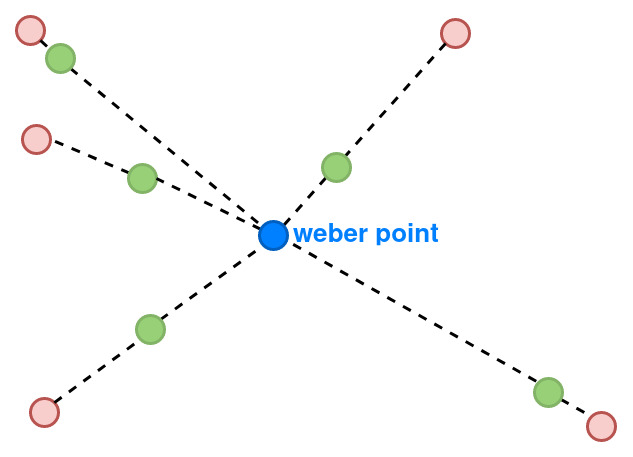
\includegraphics[width=0.7\linewidth, keepaspectratio]{figures/weber_contract}
  \end{center}
  
\end{overlayarea}
\end{frame}

\begin{frame}
\frametitle{Recap}
\begin{overlayarea}{\linewidth}{20em}
    
  \begin{itemize}
    \pause
    \item Formal proof in Coq of a simple algorithm to solve the gathering problem.
    \pause
    \item Formal proof in Coq of the properties of the weber point.
    \pause
    \item Assumes the weber point is computable.
    \pause
    \item Asynchronous and flexible setting.
    \pause
    \item Not universal : initial position must have a unique weber point.
  \end{itemize}

  \pause 
  \vspace{2em}
  \begin{center}
    \huge Thank you !
  \end{center}

\end{overlayarea}
\end{frame}
  

\end{document}